\section{The Simulation}
\label{HourglassSimulation}

\begin{frame}{Simulating The Vernier Scan}
\begin{itemize}
\item The vernier scan can be simulated with a collection of variables defining
the dynamics of the scan. We simulate each scan step, model the z-vertex
profile for the step, and modify the simulation until matching is good.

\item The goal of the hourglass simulation is to confirm that CAD has provided
the correct value for $\beta^*$ and to correct for the presence of any
crossing angle between the beams.

\item The $\beta^*$ correction was on the order of a 30\% correction in 2009,
whereas the crossing angle correction was a 1\% correction.

\item For Run 12 scans, CAD advertised the $200 GeV$ value of $\beta^*$ as $85 cm$ and the
$510 GeV$ value as $65 cm$
\end{itemize}
\end{frame}

\begin{frame}{Simulation Overview}
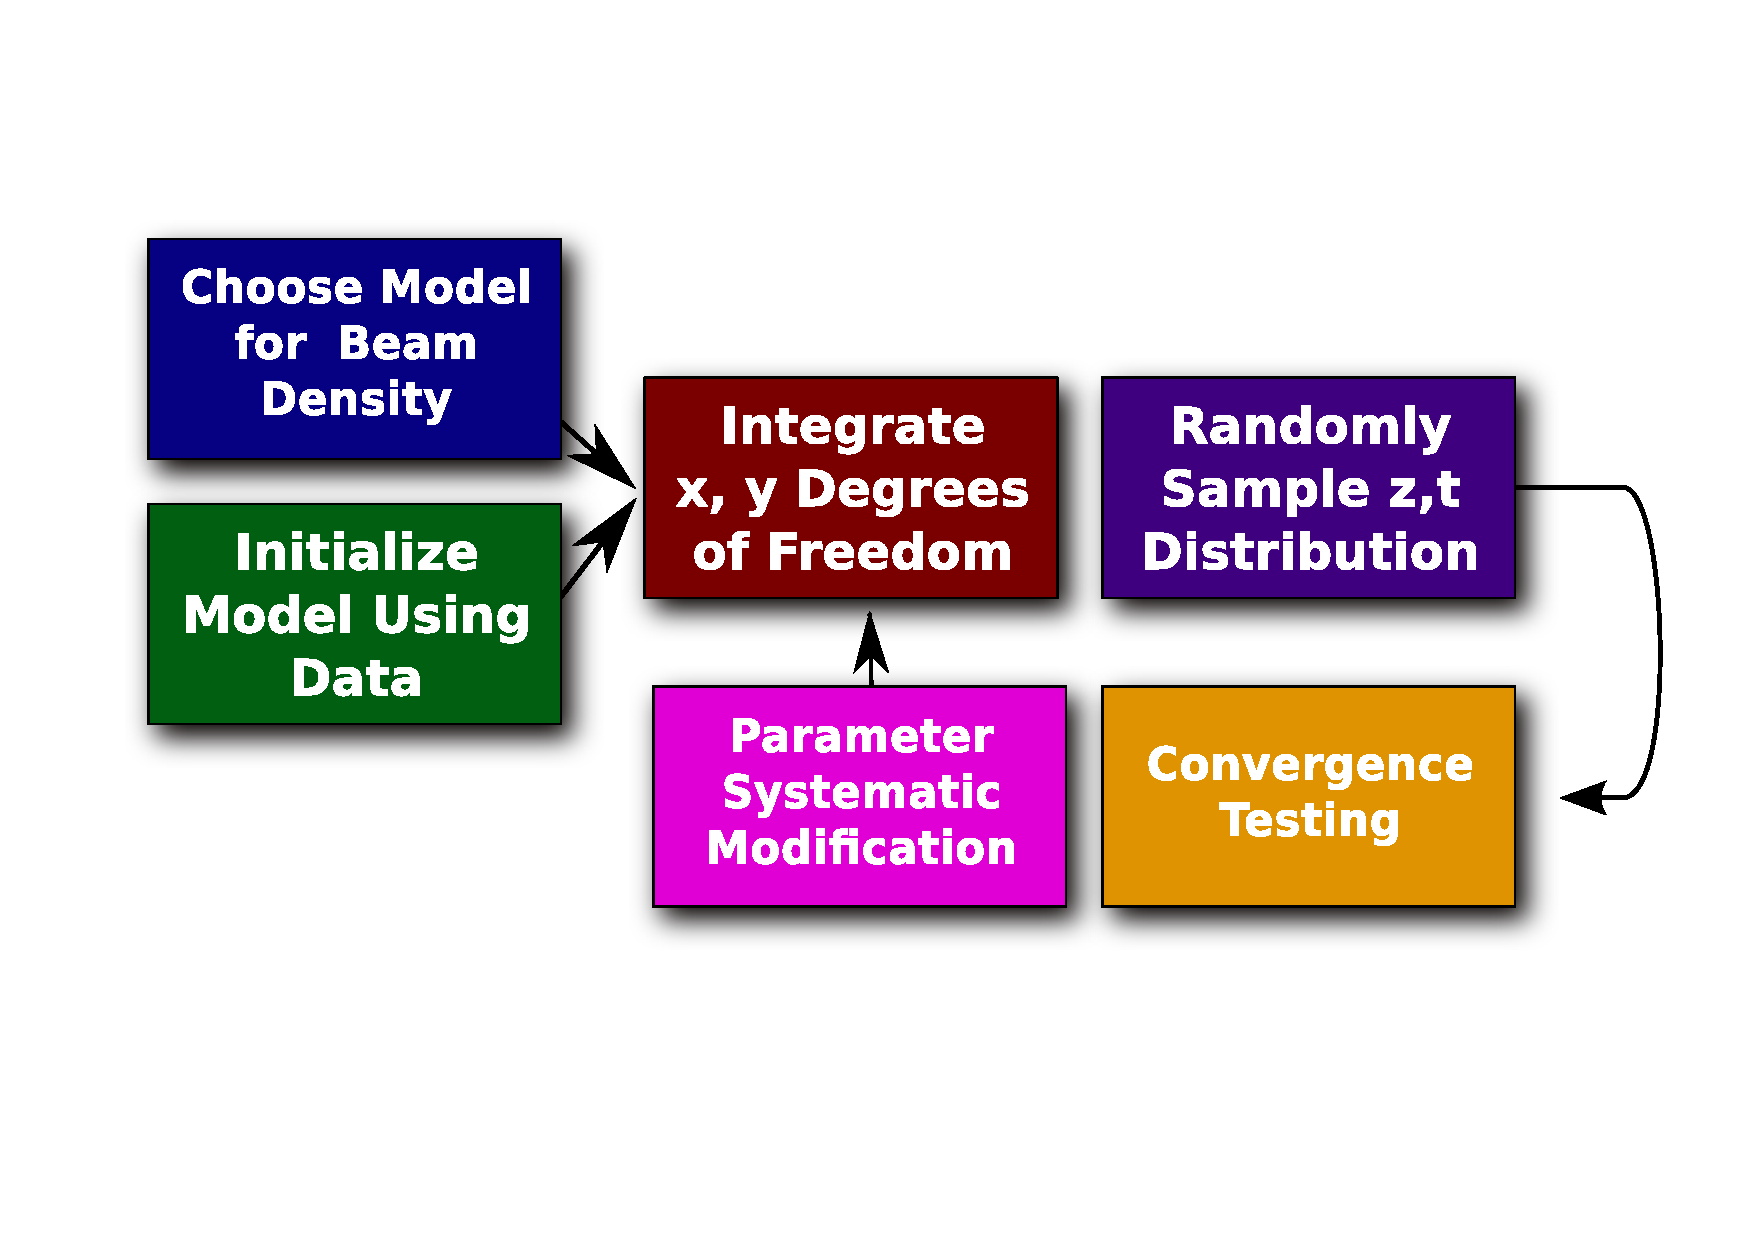
\includegraphics[height=\textheight]{../HourglassSimulation/figs/simulation_flow.pdf}
\end{frame}

\begin{frame} {Simulation Parameters}
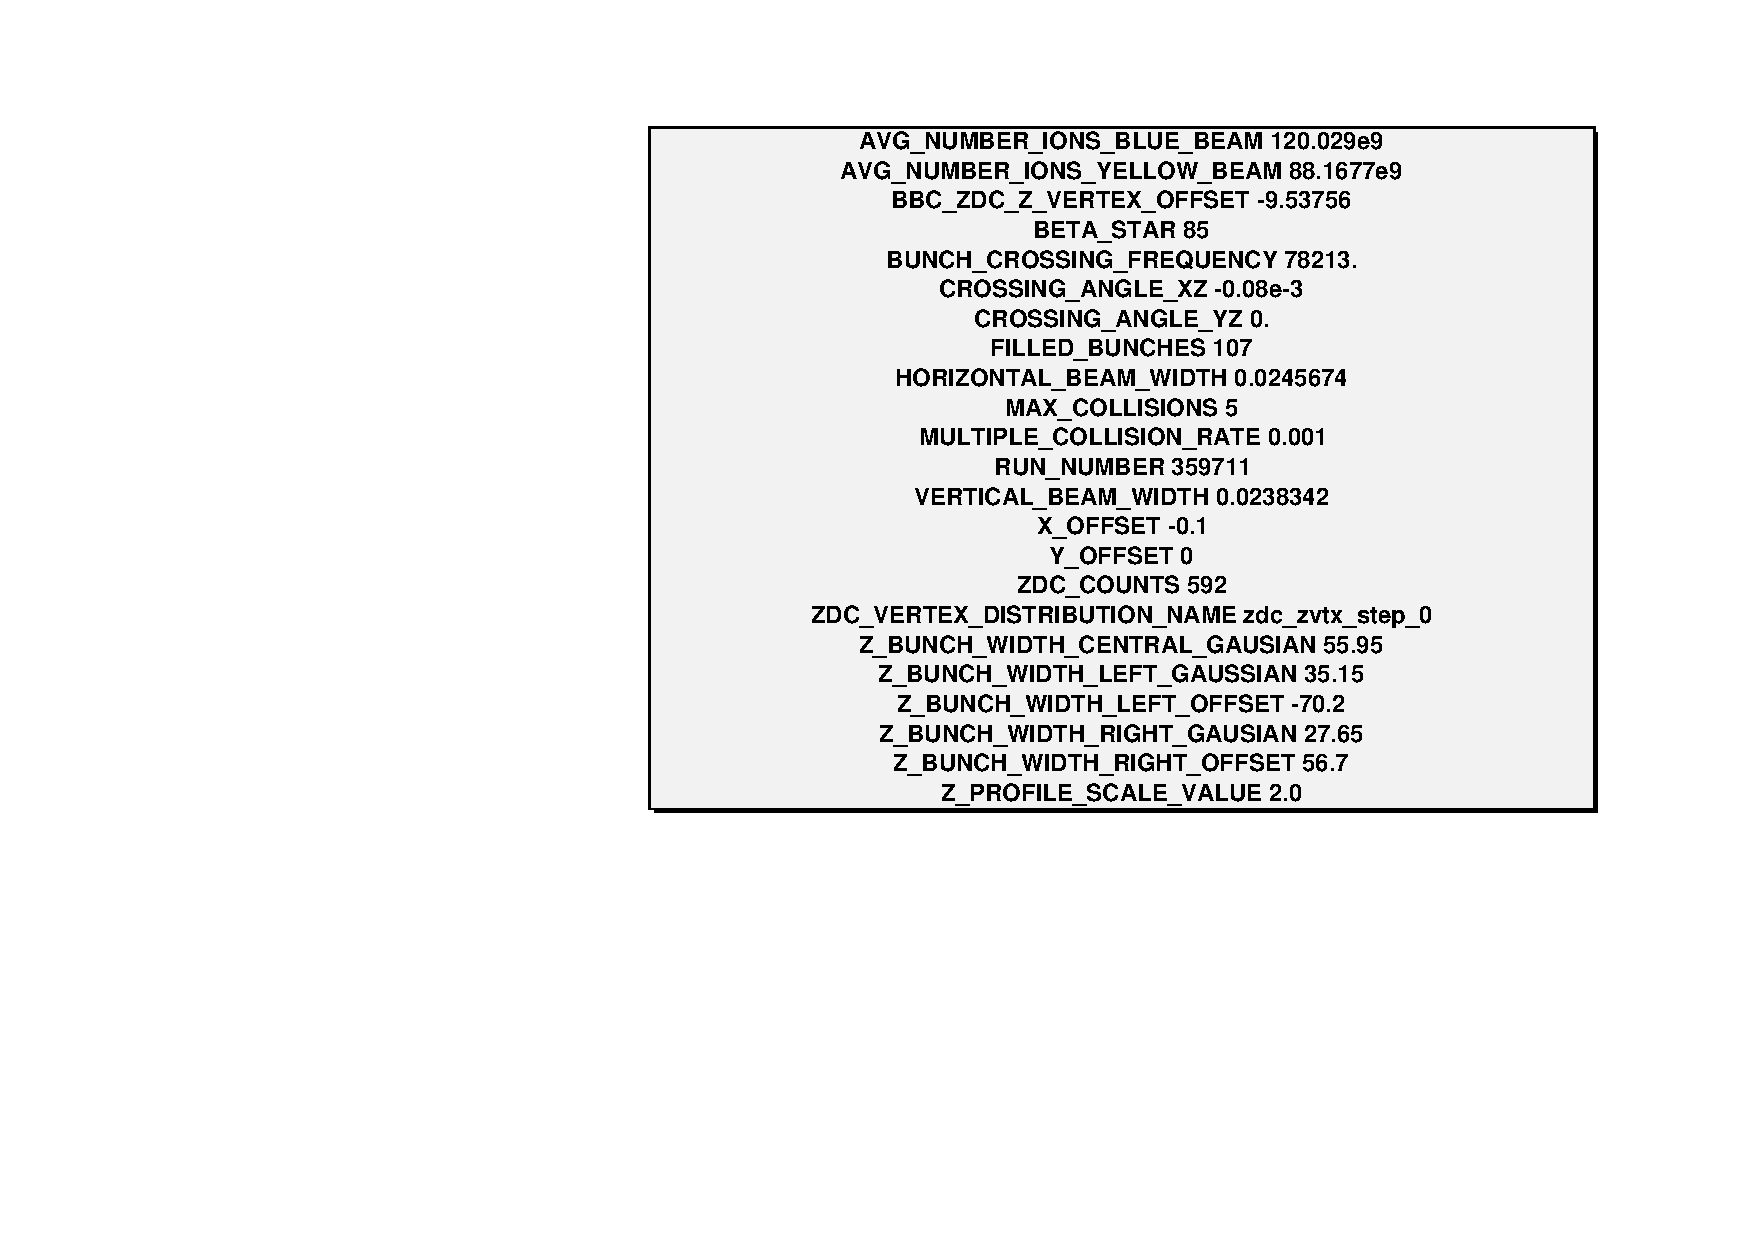
\includegraphics[width=\linewidth,height=\textheight]{../HourglassSimulation/figs/sample_configuration.pdf}
\end{frame}

\begin{frame} {Free Simulation Parameters}
Although any parameter can be varied, most are fixed based on input from other
constraints along the analysis chain.
\newline

Free parameters are:
\begin{itemize}
\item $\beta^*$
\item $\theta_{XZ}$ or $\theta_{YZ}$  
\item Z-Profile Scale value
\newline
\end{itemize}
\end{frame}

\begin{frame}{Free Simulation Parameters}
\textbf{Caveats:}
\begin{itemize}
\item Using a fixed bunch z-profile which is scaled may not be the best choice,
	but then again, the z-vertex profile may not be too sensitive to this.
	More later!
\item Crossing angle in XZ plane does not affect the shape of the z-vertex
	profile when a vertical beam displacement is simulated
\item Crossing angle in the YZ plane does not affect the shape of the z-vertex
	profile when a horizontal displacement is simulated
\item \textbf{Solution:} Simulate only one crossing angle, swap
	horizontal/vertical elements for vertical scans.
\end{itemize}

\end{frame}
